\section{First Readers-Writers Problem}
\subsection{Aim}
To implement the First Readers-Writers Problem.

\subsection{Theory}
\textbf{The problem statement}: There is a shared resource which should be accessed by
multiple processes. There are two types of processes in this context: the reader and
the writer. Any number of readers can read from the shared resource simultaneously,
but only one writer can write to the shared resource. When a writer is writing data
to the resource, no other process can access the resource. A writer cannot write to
the resource if there are non zero number of readers accessing the resource at that
time. \\
\textbf{Solution}: Here, the first reader locks the resource if such is available. Once the file
is locked from writers, it may be used by many subsequent readers without having
them to re-lock it again. \\
Before entering the critical section, every new reader must go through the entry
section. However, there may only be a single reader in the entry section at a time so
as to avoid race conditions. In order to do so, every reader which enters the ENTRY
Section will lock the ENTRY Section for themselves but does not lock the resource.
Once the reader is done executing the entry section, it will unlock it by signalling
the mutex. There can be no more than a single reader in the exit section at a time,
therefore, every reader must claim and lock the Exit section for themselves before
using it. \\
Once the first reader is in the entry section, it will lock the resource. Doing
this will prevent any writers from accessing it. Subsequent readers can just utilize
the locked resource. The very last reader must unlock the resource, thus making it
available to writers.

\subsection{Algorithm}
\begin{verbatim}
1 START
2 semaphore resource = NULL;
3 semaphore rmutex = NULL;
4 readcoun t =0;
5 procedure WRITER
6 resource.P();
7 <CRITICAL SECTION>
8 <EXIT SECTION>
9 resource.V();
10 END procedure
11 procedure READER
12 rmutex.P();
13 <CRITICAL SECTION>
14 readcoun t++;
15 IF readcoun t == 1 THEN
16 resource.P();
17 END IF
18 <EXIT CRITICAL SECTION>
19 rmutex.V();
20 rmutex.P();
21 <CRITICAL SECTION>
22 readcount −−;
23 IF readcoun t == 0 THEN
24 resource.V();
25 END IF
26 <EXIT CRITICAL SECTION>
27 rmutex.V();
28 END procedure
29 STOP
\end{verbatim}

\subsection{Source Code}
\subsubsection{Ordinary pipe}
\begin{lstlisting}[language=C]
#include <stdio.h>
#include <semaphore.h>
#include <pthread.h>

#define NO_OF_READERS 3
#define NO_OF_WRITERS 2

static sem_t write_lock; // Semaphore for updating and signalling
static pthread_mutex_t n_reader_lock; // Mutex for editing number of readers
static int n_reader = 0; // Number of readers at a certain instance of time
static int data = 100; // Data to be read

void *reader_start_routine(void *tid) {
  int thread_id = *((int *) tid);

  printf(
    "[Reader%d]: Waiting to acquire lock for incrementing n_reader\n", 
    thread_id
  );
  pthread_mutex_lock(&n_reader_lock);

  printf("[Reader%d]: Updating n_reader\n", thread_id);
  ++n_reader;
  if(n_reader == 1) {
    printf("[Reader%d]: First reader. Acquiring write lock\n", thread_id);
    sem_wait(&write_lock);
  }

  printf("[Reader%d]: Unlocking n_reader lock\n", thread_id);
  pthread_mutex_unlock(&n_reader_lock);

  printf("[Reader%d]: Read value: %d\n", thread_id, data);

  printf(
    "[Reader%d]: Waiting to acquire lock for decrementing n_reader\n", 
    thread_id
  );
  pthread_mutex_lock(&n_reader_lock);

  printf("[Reader%d]: Updating n_reader\n", thread_id);
  --n_reader;
  if(n_reader == 0) {
    printf(
      "[Reader%d]: No readers left. Unlocking write lock\n", 
      thread_id
    );
    sem_post(&write_lock);
  }

  printf("[Reader%d]: Unlocking n_reader lock\n", thread_id);
  pthread_mutex_unlock(&n_reader_lock);
}

void *writer_start_routine(void *tid) {
  int thread_id = *((int *) tid);

  printf("[Writer%d]: Waiting for write lock\n", thread_id);
  sem_wait(&write_lock);

  printf(
    "[Writer%d]:Write lock acquired. Incrementing value\n",
    thread_id
  );
  ++data;

  printf("[Writer%d]: Unlocking write lock\n", thread_id);
  sem_post(&write_lock);
}

int main() {
  pthread_t readers[NO_OF_READERS], writers[NO_OF_WRITERS];
  int reader_ids[NO_OF_READERS], writer_ids[NO_OF_WRITERS];
  
  sem_init(&write_lock, 0, 1);

  // Generating unique identifiers for threads
  for(int i = 0; i < NO_OF_READERS; reader_ids[i++] = i); 
  for(int i = 0; i < NO_OF_WRITERS; writer_ids[i++] = i); 
  
  for(int i = 0; i < NO_OF_READERS; i++) 
    pthread_create(
      &readers[i], 
      NULL, 
      reader_start_routine, 
      (void *)&reader_ids[i]
    );
  
  for(int i = 0; i < NO_OF_WRITERS; i++)
    pthread_create(
      &writers[i], 
      NULL, 
      writer_start_routine, 
      (void *)&writer_ids[i]
    );

  for(int i = 0; i < NO_OF_READERS; i++) 
    pthread_join(readers[i], NULL);

  for(int i = 0; i < NO_OF_WRITERS; i++)
    pthread_join(writers[i], NULL);

  return 0;
}



\end{lstlisting}

\begin{center}
	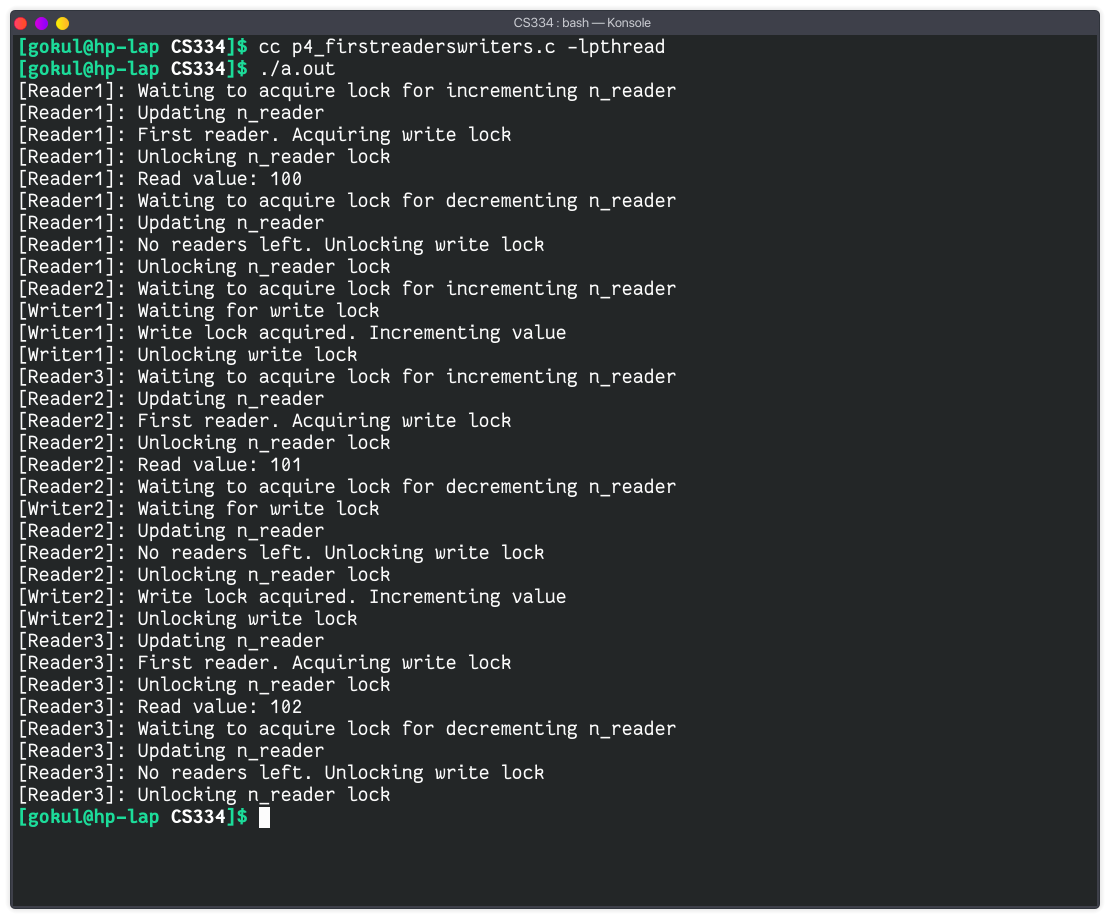
\includegraphics[width=0.90\textwidth]{img/p5.png}
\end{center}


\subsection{Result}
The above programs were executed and its output were verified